\begin{frame}
    \frametitle{Grafo}

    Las bases de datos en grafo utilizan estructuras de grafo para almacenar, consultar y relacionar datos. 

    \begin{center}
    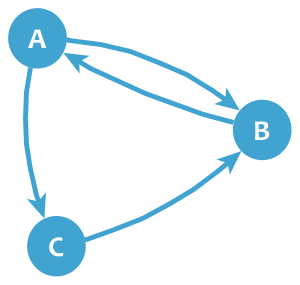
\includegraphics[width=0.2\textwidth]{diagramas/Grafo.png}
    \end{center}
    
     
    
    Los datos se representan mediante nodos (entidades) y arcos (relaciones entre entidades).  
    
    Pueden asignarse propiedades a nodos y arcos para capturar más detalles.
\end{frame}

\begin{frame}
    \frametitle{Grafo - Casos de uso}

    Las bases de datos en grafo son ideales para almacenar datos interconectados.  
    Aplicaciones comunes incluyen:
    \begin{itemize}
        \item Redes sociales\\
          
        \item Sistemas de recomendación\\
         
        \item Redes de trasportes\\
        
    \end{itemize}

    Los datos almacenados pueden interpretarse de diferentes maneras basadas en las relaciones entre los nodos.
\end{frame}

\begin{frame}
    \frametitle{Grafo - Desventajas}
    \begin{itemize}
        \item Las bases de datos en grafo presentan complejidad de modelado y un costo de aprendizaje elevado para usuarios no familiarizados.

         

        \item Pueden experimentar dificultades de rendimiento y requerir esfuerzos adicionales de mantenimiento y optimización.
    \end{itemize}
\end{frame}


\begin{frame}
    \frametitle{Grafo - Ejemplos}
    Algunos ejemplos de bases de datos en grafos son:
    
     

    \begin{itemize}
        \item \textbf{Neo4J}\\
        Una de las bases de datos en grafo más populares y utilizadas en la industria. Ofrece una gran variedad de herramientas y bibliotecas para el modelado y análisis de grafos.

         

        \item \textbf{GraphBase}\\ 
        Un sistema que permite crear y consultar grafos de datos, con capacidades avanzadas para el análisis de datos.

         
        
        \item \textbf{Infinite Graph}\\
        Ofrece una plataforma para trabajar con grafos a gran escala, con soporte para consultas complejas y análisis de grafos.    
        
         

        \item \textbf{FlockDB}\\
        Un sistema de bases de datos en grafo diseñado para manejar relaciones entre grandes volúmenes de datos, con un enfoque en el rendimiento y la escalabilidad.
    \end{itemize}
    
\end{frame}